\documentclass[12pt,a4paper]{article}

%--------------------------------
% PAQUETES
%--------------------------------
\usepackage[spanish]{babel}
\usepackage[utf8]{inputenc}
\usepackage[T1]{fontenc}
\usepackage{geometry}
\usepackage{graphicx}
\usepackage{float}
\usepackage{amsmath}
\usepackage{hyperref}

\geometry{margin=2.5cm}

%--------------------------------
% DATOS DEL INFORME (COMPLETAR)
%--------------------------------

%--------------------------------
\begin{document}

%--------------------------------
% PORTADA
%--------------------------------
\begin{titlepage}
    \centering

    {\scshape\LARGE Universidad Tecnológica Nacional \par}
    \vspace{0.3cm}
    {\scshape\Large Facultad Regional Córdoba \par}
    \vspace{1.5cm}

    {\scshape\Large Analisis de señales y sistemas \par}
    \vspace{2cm}

    {\Huge\bfseries Trabajo Práctico N°1 \par}
    
    \vspace{2cm}

    \begin{flushleft}
    \textbf{Integrantes:} \\
    Nombre y Apellido -- Legajo \\
    Nombre y Apellido -- Legajo \\
    Nombre y Apellido -- Legajo \\

    \vspace{0.5cm}

    \textbf{Curso:} 3R\_X \\
    \textbf{Grupo:} XX \\
    \textbf{Docente:} --- \\
    \textbf{Año:} 2026 \\
    \end{flushleft}

    \vfill

\end{titlepage}
\thispagestyle{empty}

\vspace{1cm}

\tableofcontents
\newpage

%--------------------------------
\section {Introducción}
%--------------------------------


\vspace{0.5cm}



% ============================================================
\section{Ejercicio 1}
% ============================================================
 
Se considera la función en variable compleja:
\[
    f(z) = \sin\!\left(e^{j\pi/2} \cdot z^{2}\right)
\]
 
% ------------------------------------------------------------
\subsection {a) Conjunto de ceros $S$: $f(z) = 0$}
% ------------------------------------------------------------
 
\begin{align*}
    \sin\!\left(e^{j\pi/2} \cdot z^{2}\right) &= 0 \\[6pt]
    \Rightarrow \quad e^{j\pi/2} \cdot z^{2} &= n\pi, \quad n \in \mathbb{Z} \\[6pt]
    \Rightarrow \quad z^{2} &= n\pi \cdot e^{-j\pi/2} \\[6pt]
    \Rightarrow \quad z &= \sqrt{n\pi} \cdot e^{-j\pi/4}, \quad \forall\, n \in \mathbb{Z}
\end{align*}
 
Escribiendo $z = x + jy$ con $z = \text{Re}(z) + j\,\text{Im}(z)$:
 
\[
    \begin{cases}
        x = \sqrt{n\pi} \cdot \cos\!\left(-\tfrac{\pi}{4}\right) \\[4pt]
        y = \sqrt{n\pi} \cdot \sin\!\left(-\tfrac{\pi}{4}\right)
    \end{cases}
    \quad \Rightarrow \quad \sqrt{n\pi} \in \mathbb{R}
\]
 
% ------------------------------------------------------------
\subsection {b) Demostración de que $S$ es un conjunto con infinitos ceros sobre $S_1$ y $S_2$}
% ------------------------------------------------------------
 
Se definen las rectas paramétricas:
\[
    S_1 = \left\{ t\, e^{-j\pi/4} : t \in \mathbb{R} \right\}, \qquad
    S_2 = \left\{ t\,j\, e^{-j\pi/4} : t \in \mathbb{R} \right\}
\]
 
\textbf{Análisis del Conjunto $S_1$:}
 
\begin{align*}
    t \cdot e^{-j\pi/4}
    &= t\left[\cos\!\left(-\tfrac{\pi}{4}\right) + j\,\sin\!\left(-\tfrac{\pi}{4}\right)\right]
     = t\left(\frac{\sqrt{2}}{2}\right) + j\, t\left(-\frac{\sqrt{2}}{2}\right)
\end{align*}
 
Sea $z = x + jy$, entonces por analogía:
\[
    x = t\!\left(\frac{\sqrt{2}}{2}\right), \qquad y = t\!\left(-\frac{\sqrt{2}}{2}\right)
    \quad \Rightarrow \quad x = y, \quad \forall\, t \in \mathbb{R}
\]
 
Sabiendo que el modelo de una recta es $y = ax + b$, por analogía se trata de una recta
de pendiente $a = 1$ y ordenada al origen $b = 0$.
 
\medskip
\textbf{Análisis del Conjunto $S_2$:}
 
\begin{align*}
    t \cdot j \cdot e^{-j\pi/4}
    &= t \cdot j \cdot \cos\!\left(-\tfrac{\pi}{4}\right) - t \cdot \sin\!\left(-\tfrac{\pi}{4}\right) \\
    &= t \cdot j \cdot \frac{\sqrt{2}}{2} - t\!\left(-\frac{\sqrt{2}}{2}\right)
     = t\!\left(\frac{\sqrt{2}}{2}\right) + j\left[-t\!\left(\frac{\sqrt{2}}{2}\right)\right]
\end{align*}
 
% Nota: la parte real es t*(sqrt(2)/2) y la imaginaria es -t*(sqrt(2)/2), por lo que -x = y
Por analogía: $-x = y$, es decir, recta de pendiente $a = -1$ y ordenada al origen $b = 0$.
 
\bigskip
\textbf{Verificación de que los ceros de $S$ caen sobre $S_1$:}
 
Sea $z = t \cdot e^{-j\pi/4}$:
\begin{align*}
    z^2 &= t^2 \cdot e^{-j\pi/2} = t^2 \cdot (-j) \\
    \Rightarrow \quad j z^2 &= t^2
\end{align*}
Sustituyendo en la ecuación de ceros: $e^{j\pi/2} \cdot z^2 = t^2$, luego:
\[
    \sin(t^2) = 0 \quad \Rightarrow \quad t^2 = \sqrt{n\pi} \qquad \text{(discreto)}
\]
 
\textbf{Verificación de que los ceros de $S$ caen sobre $S_2$:}
 
Sea $z = t \cdot j \cdot e^{-j\pi/4}$:
\begin{align*}
    z^2 &= t^2 \cdot j^2 \cdot e^{-j\pi/2} = t^2 \cdot (-1) \cdot (-j) = t^2 \cdot j \\
    \Rightarrow \quad e^{j\pi/2} \cdot z^2 &= -t^2
\end{align*}
Luego:
\[
    \sin(-t^2) = 0 \quad \Rightarrow \quad -t^2 = \sqrt{n\pi} \qquad \text{(discreto)}
\]


 \begin{figure}[H]
    \centering
    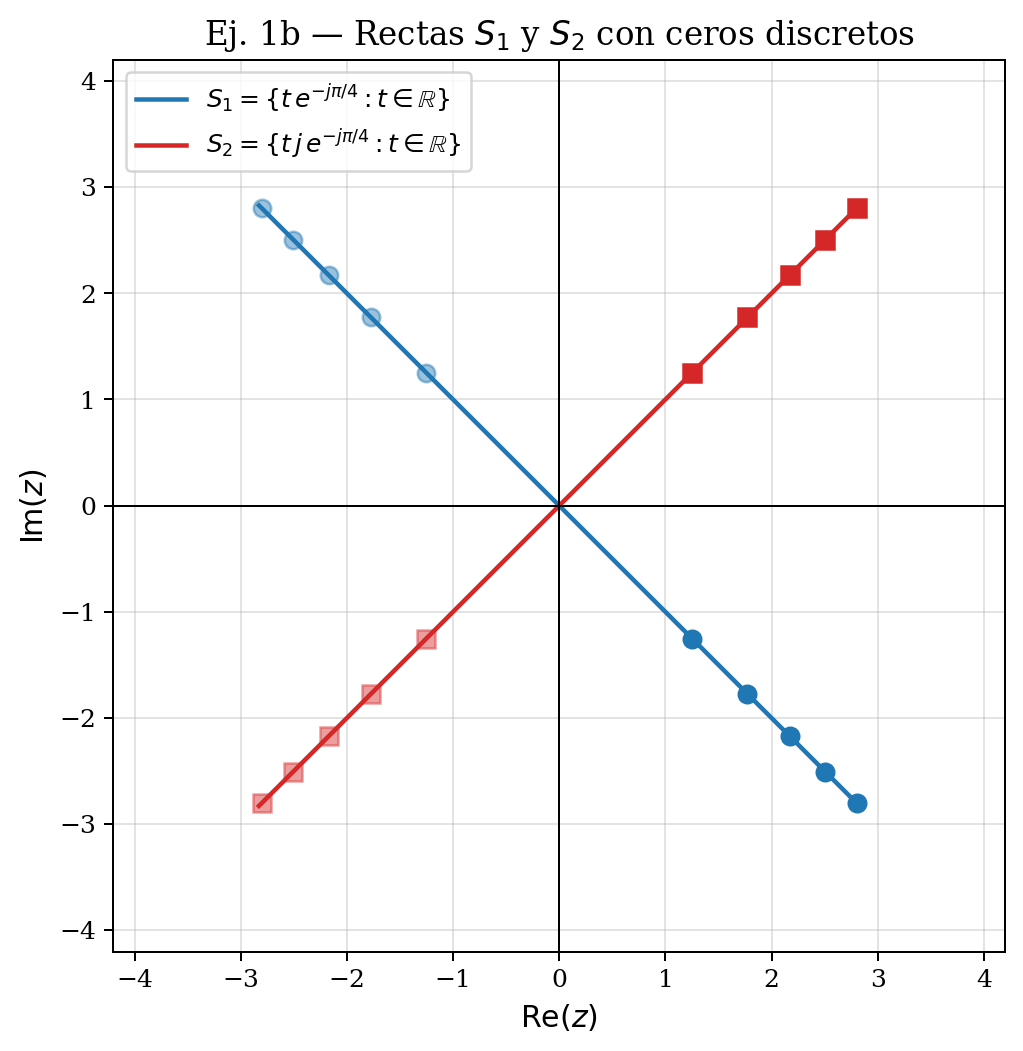
\includegraphics[width=0.6\textwidth]{ej1b_rectas.png}
\end{figure}
% Nota: ambos conjuntos $S_1$ y $S_2$ son discretos porque los valores de t que satisfacen
% la ecuación son aislados (raíces cuadradas de múltiplos de pi).
 
% ------------------------------------------------------------
\subsection {c) Módulos y argumentos de $S_1 = S \cap \{t\,e^{-j\pi/4} : t \in \mathbb{R}\}$}
% ------------------------------------------------------------
 
Para $z = t \cdot e^{-j\pi/4}$, los elementos del conjunto discreto son:
 
\begin{align*}
    t = 1 &\;\Rightarrow\; z = 1 \cdot e^{-j\pi/4} & |z| &= 1, & \operatorname{Arg}(z) &= -\frac{\pi}{4} \\[4pt]
    t = 2 &\;\Rightarrow\; z = 2 \cdot e^{-j\pi/4} & |z| &= 2, & \operatorname{Arg}(z) &= -\frac{\pi}{4}
\end{align*}
 
En general:
\[
    |z| = t, \qquad \operatorname{Arg}(z) = -\frac{\pi}{4}
\]


 
 \begin{figure}[H]
    \centering
    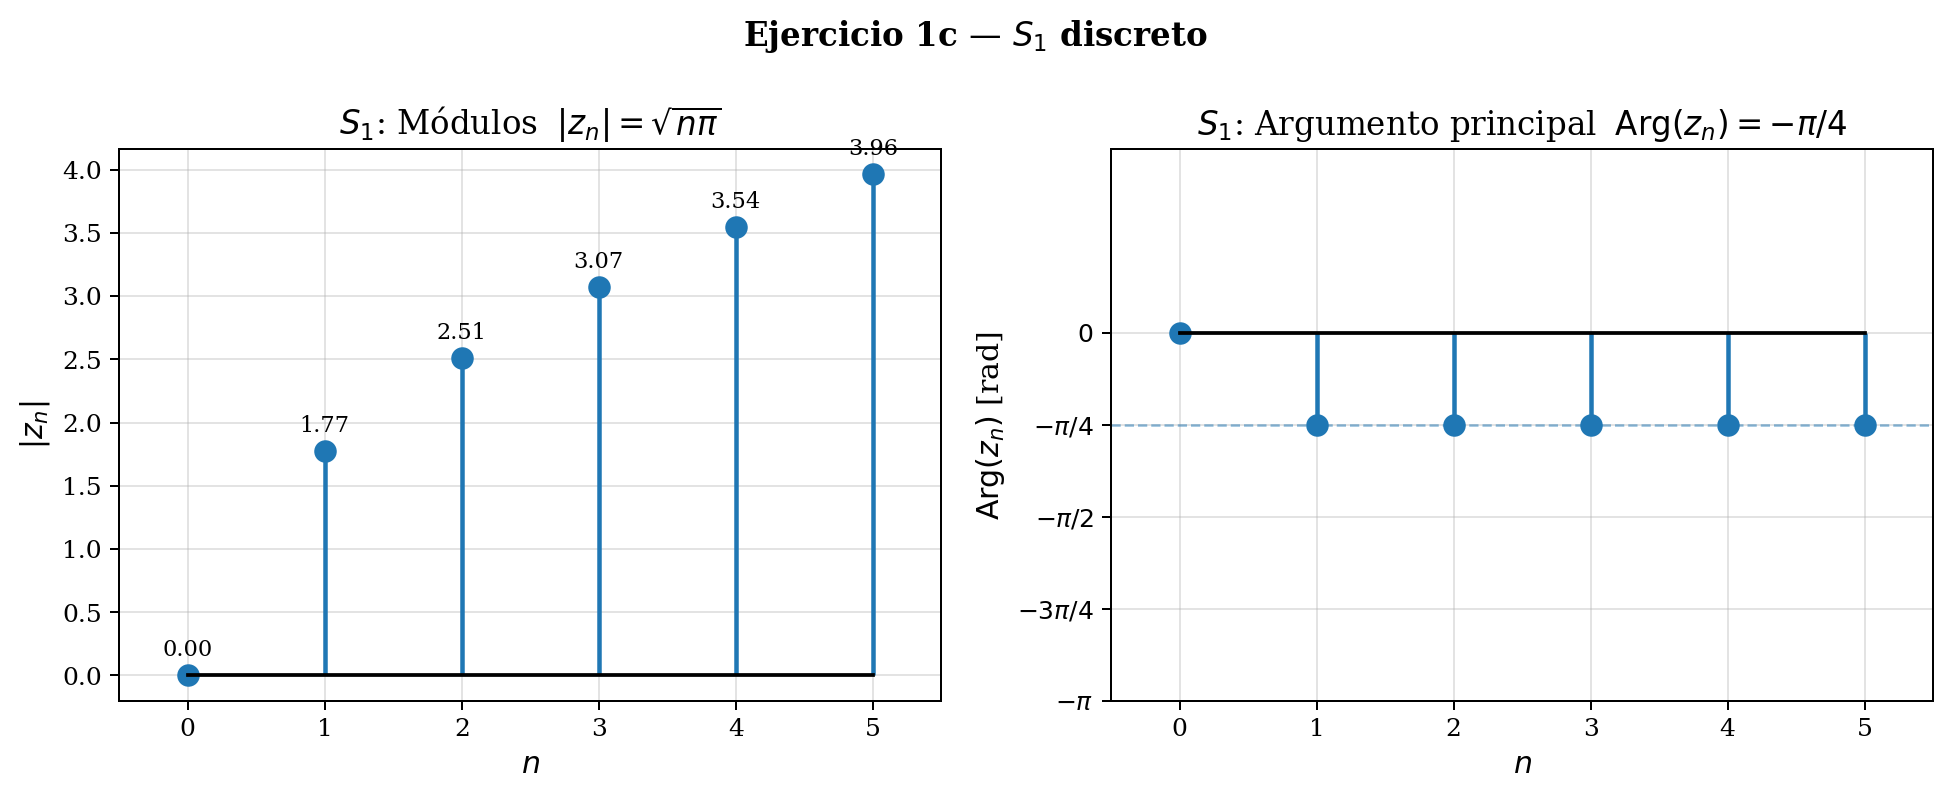
\includegraphics[width=0.9\textwidth]{ej1c_S1.png}
\end{figure}

% Nota: el argumento es constante para todos los elementos; lo que varía es el módulo.
% Se debe graficar: (1) módulo vs índice n, (2) argumento (constante en -pi/4) vs índice n.
% [GRAFICAR --- pendiente]
 
% ------------------------------------------------------------
\subsection {d) Módulos y argumentos de $S_2 = S \cap \{t\,j\,e^{-j\pi/4} : t \in \mathbb{R}\}$}
% ------------------------------------------------------------
 
Para $z = t \cdot j \cdot e^{-j\pi/4}$:
\begin{align*}
    j \cdot e^{-j\pi/4} &= e^{j\pi/2} \cdot e^{-j\pi/4} = e^{j(\pi/2 - \pi/4)} = e^{j\pi/4}
\end{align*}
 
Entonces $z = t \cdot e^{j\pi/4}$, y los elementos son:
 
\begin{align*}
    t = 1 &\;\Rightarrow\; z = e^{j\pi/4}     & |z| &= 1, & \operatorname{Arg}(z) &= \frac{\pi}{4} \\[4pt]
    t = 2 &\;\Rightarrow\; z = 2\,e^{j\pi/4}  & |z| &= 2, & \operatorname{Arg}(z) &= \frac{\pi}{4}
\end{align*}
 
En general:
\[
    |z| = t, \qquad \operatorname{Arg}(z) = \frac{\pi}{4}
\]
 
% Nota: análogamente al inciso c), el argumento es constante (pi/4) y el módulo crece.
% [GRAFICAR --- pendiente]
\begin{figure}[H]
    \centering
    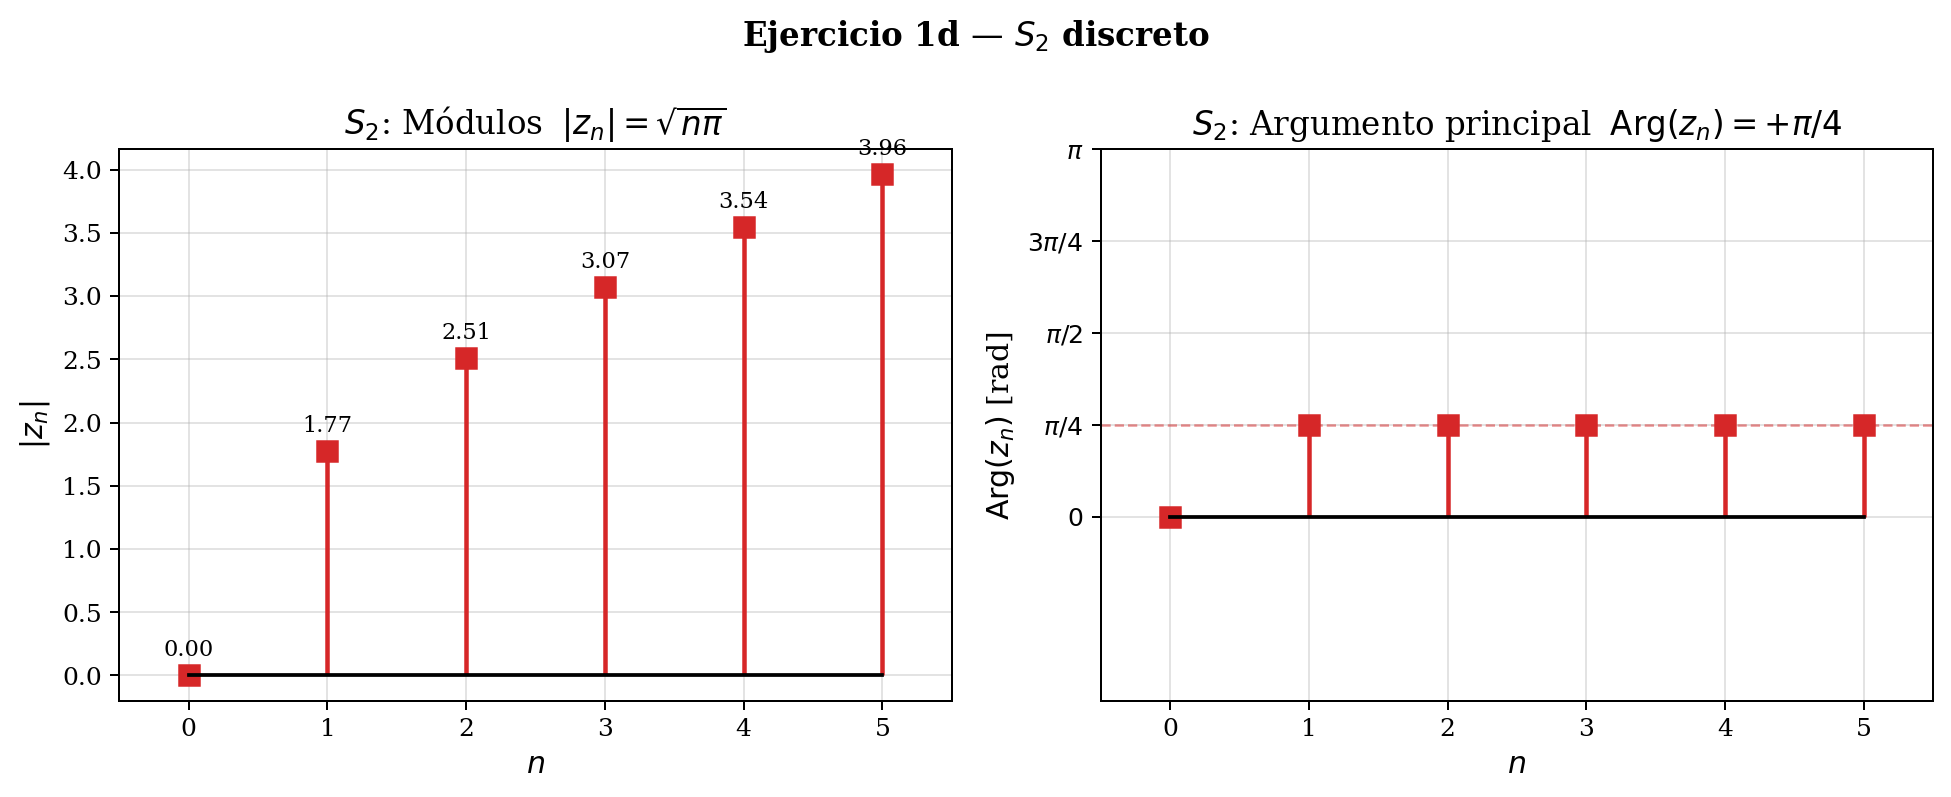
\includegraphics[width=0.6\textwidth]{ej1d_S2.png}
\end{figure}



% ============================================================
\section {Ejercicio 2}
% ============================================================
 
Se considera la relación entre variables complejas $z, w \in \mathbb{C}$:
\[
    z = \frac{4w + 8}{w - 1}
\]
 
% ------------------------------------------------------------
\subsection {a) Despejar $w = f(z)$ y calcular $\lim_{z \to \infty} f(z)$}
% ------------------------------------------------------------
 
\begin{align*}
    z(w - 1) &= 4w + 8 \\
    zw - z   &= 4w + 8 \\
    zw - 4w  &= z + 8 \\
    w(z - 4) &= z + 8 \\[6pt]
    \Aboxed{w = f(z) &= \frac{z + 8}{z - 4}}
\end{align*}
 
\[
    \lim_{z \to \infty} f(z) = \lim_{z \to \infty} \frac{z + 8}{z - 4} = 1
\]
 
% ------------------------------------------------------------
\subsection {b) Forma rectangular $f(z) = u(x,y) + j\,v(x,y)$}
% ------------------------------------------------------------
 
% Nota: en el manuscrito no se desarrolla explícitamente la forma rectangular.
% A continuación se reconstruye el procedimiento estándar a partir de z = x + jy.
 
Sea $z = x + jy$:
\begin{align*}
    f(z) &= \frac{(x+jy) + 8}{(x+jy) - 4}
           = \frac{(x+8) + jy}{(x-4) + jy}
\end{align*}
 
Multiplicando numerador y denominador por el conjugado del denominador:
\begin{align*}
    f(z) &= \frac{\left[(x+8)+jy\right]\left[(x-4)-jy\right]}{(x-4)^2 + y^2}
\end{align*}
 
\begin{align*}
    u(x,y) &= \frac{(x+8)(x-4) + y^2}{(x-4)^2 + y^2} \\[6pt]
    v(x,y) &= \frac{y(x-4) - y(x+8)}{(x-4)^2 + y^2}
             = \frac{-12y}{(x-4)^2 + y^2}
\end{align*}
 
% ------------------------------------------------------------
\subsection {c) Mapeo de la región $|z - 4| \leq 1$ mediante $w = f(z)$}
% ------------------------------------------------------------
 
\textbf{Región en el plano $Z$:} disco centrado en $z_0 = 4$, radio $r = 1$.
 
\textbf{Obtención de la región imagen en el plano $W$:}
 
Se parte de:
\[
    |z - 4| \leq 1
\]
 
A partir de $w = \dfrac{z+8}{z-4}$, se despeja $z - 4$:
 
\begin{align*}
    z - 4 &= \frac{12}{w - 1}
    % Verificación: z-4 = (z+8)/(w-... se deduce de z-4 = 4w+8 - 4(w-1)/(w-1) = 12/(w-1)
\end{align*}

Verificación: z-4 = [(z+8)/w] se deduce de z-4 = 4w+8 - 4(w-1)/(w-1) = 12/(w-1)\\
 
Entonces:
\[
    |z - 4| = \frac{12}{|w - 1|} \leq 1
\]
 
\[
    \frac{12}{|w - 1|} \leq 1 \quad \Rightarrow \quad 12 \leq |w - 1|
\]
 
Escribiendo $w = u + jv$:
\[
    \frac{12}{\sqrt{(u-1)^2 + v^2}} \leq 1
    \quad \Rightarrow \quad
    12 \leq \sqrt{(u-1)^2 + v^2}
    \quad \Rightarrow \quad
    144 \leq (u-1)^2 + v^2
\]
 
\[
    \boxed{(u-1)^2 + v^2 \geq 144}
\]
 
\textbf{Conclusión:} El disco $|z-4| \leq 1$ se mapea al \emph{exterior} del disco
centrado en $w_0 = 1$ con radio $R = 12$ en el plano $W$.
 
% [GRAFICAR ambos dominios --- pendiente]
 \begin{figure}[H]
    \centering
    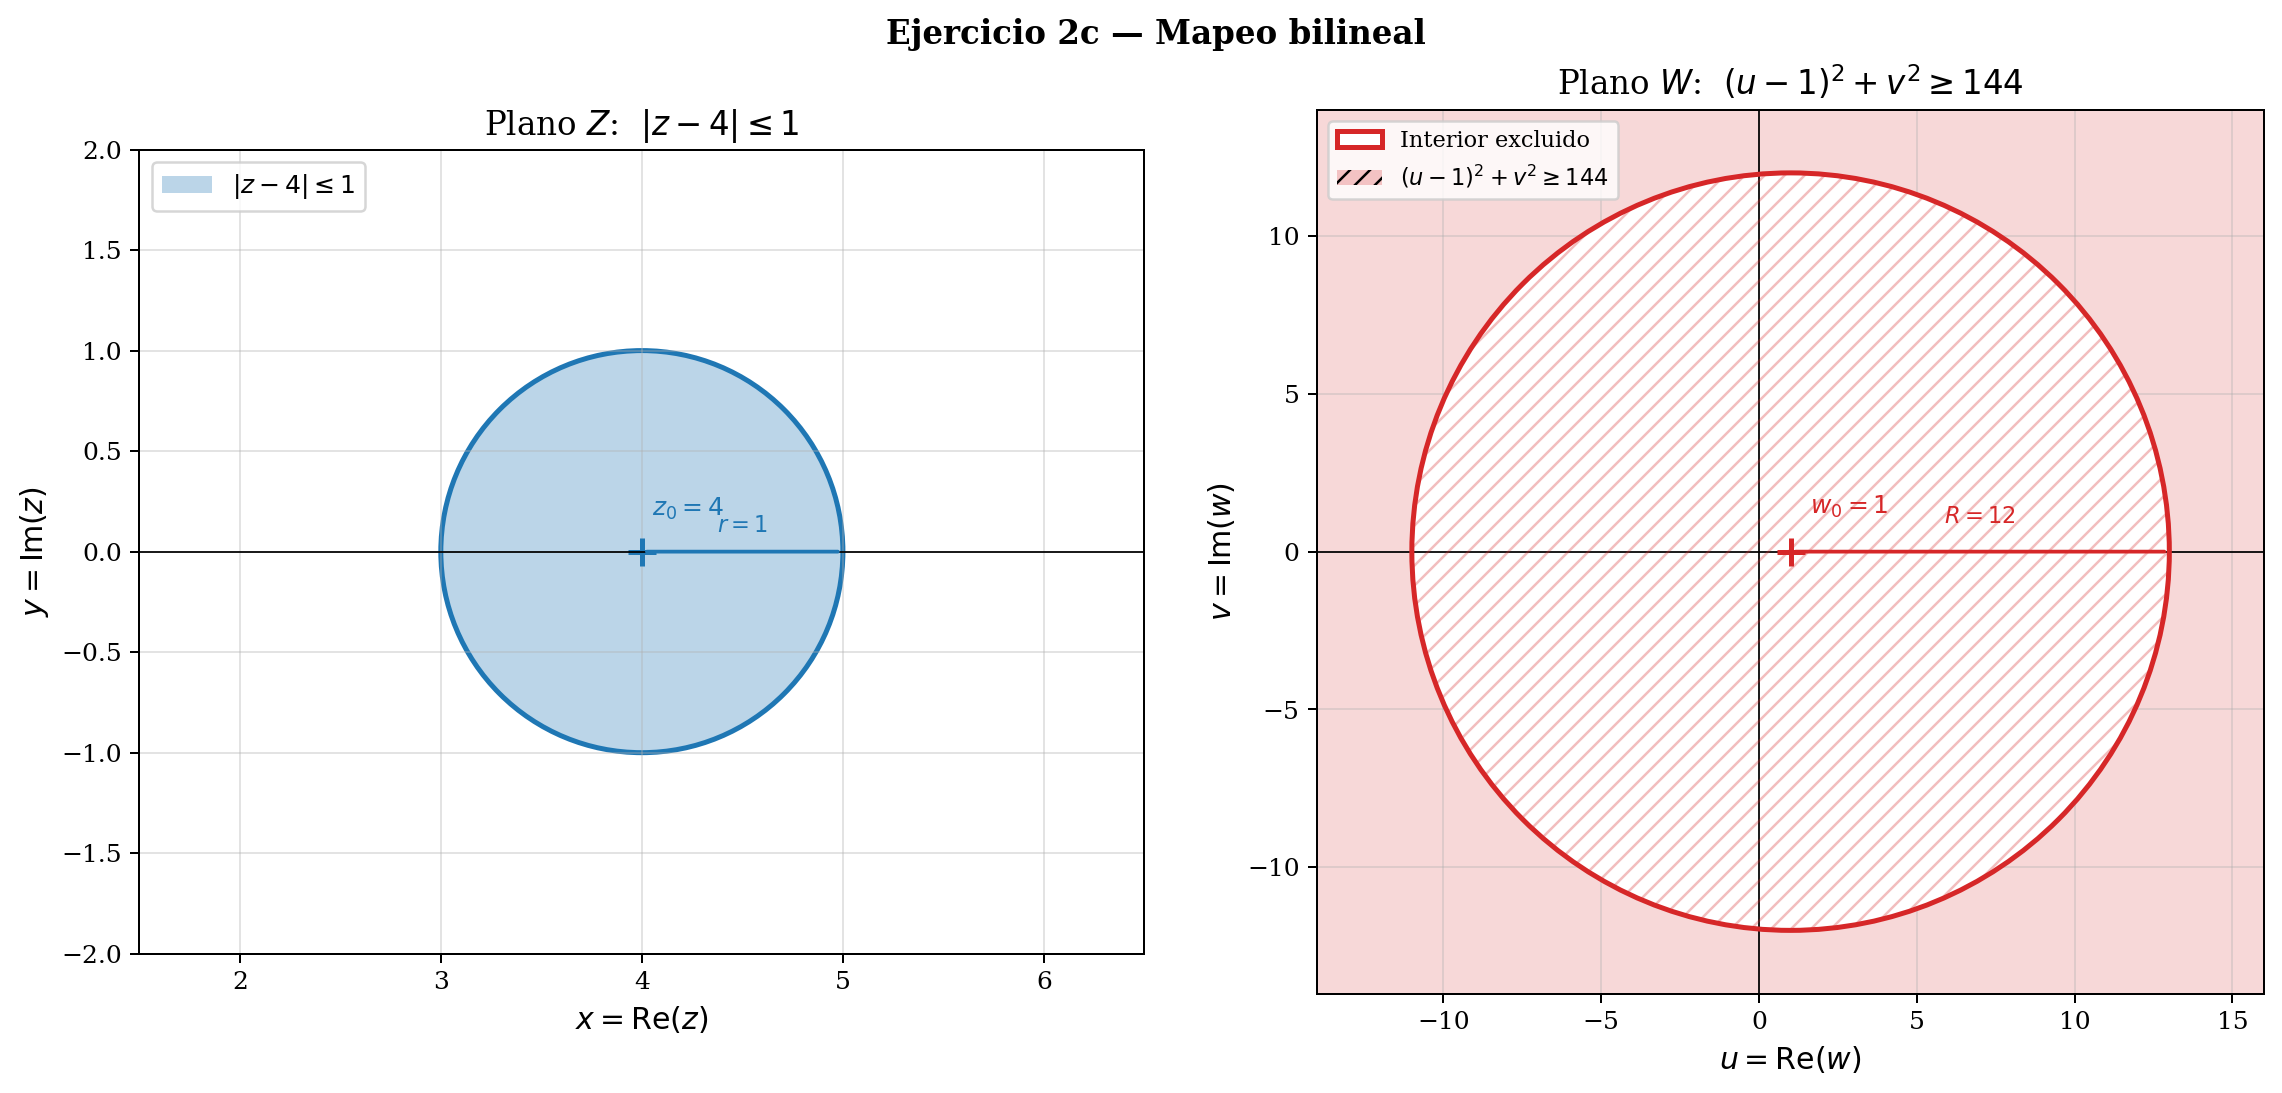
\includegraphics[width=0.6\textwidth]{ej2c_mapeo.png}
\end{figure}

 
% ============================================================
\section {Ejercicio 3}
% ============================================================
 
% ------------------------------------------------------------
\subsection {b) Ecuación cuadrática: $3z^2 + (2 - 3j)z - 1 - 3j = 0$}
% ------------------------------------------------------------
 
Se divide por $3$:
\[
    z^2 + \left(\frac{2}{3} - j\right)z - \frac{1}{3} - j = 0
\]
 
Aplicando la fórmula cuadrática $z = \dfrac{-b \pm \sqrt{b^2 - 4ac}}{2a}$ con
$a = 3,\; b = (2-3j),\; c = (-1-3j)$:
 
\[
    z = \frac{-\left(\frac{2}{3} - j\right) \pm \sqrt{\left(\frac{2}{3} - j\right)^2 - 4\cdot\left(-\frac{1}{3} - j\right)}}{2}
\]
 
\textbf{Cálculo del discriminante:}
 
\begin{align*}
    \left(\frac{2}{3} - j\right)^2 &= \frac{4}{9} - \frac{4j}{3} - 1
                                    = -\frac{5}{9} - \frac{4j}{3}
                                    % = 4/9 - 4j/3 + j^2 = 4/9 - 4j/3 - 1
\end{align*}
 
\begin{align*}
    -4\left(-\frac{1}{3} - j\right) &= \frac{4}{3} + 4j
\end{align*}
 
\begin{align*}
    \Delta &= -\frac{5}{9} - \frac{4j}{3} + \frac{4}{3} + 4j
            = \left(-\frac{5}{9} + \frac{12}{9}\right) + j\left(-\frac{4}{3} + 4\right)
            = \frac{7}{9} + j\,\frac{8}{3}
\end{align*}
 
% Nota: en el manuscrito se obtiene 8/3j + 7/9. Coincide con lo calculado.
 
\textbf{Conversión a forma polar de $\Delta = \dfrac{7}{9} + j\dfrac{8}{3}$:}
 
\textbf{Cálculo del discriminante:}

\begin{align*}
    \left(\frac{2}{3} - j\right)^2 &= \frac{4}{9} - \frac{4j}{3} - 1
                                    = -\frac{5}{9} - \frac{4j}{3}
\end{align*}

\begin{align*}
    -4\left(-\frac{1}{3} - j\right) &= \frac{4}{3} + 4j
\end{align*}

\begin{align*}
    \Delta &= -\frac{5}{9} - \frac{4j}{3} + \frac{4}{3} + 4j
            = \left(-\frac{5}{9} + \frac{12}{9}\right) + j\left(-\frac{4}{3} + 4\right)
            = \frac{7}{9} + j\,\frac{8}{3}
\end{align*}

\textbf{Conversión a forma polar de $\Delta = \dfrac{7}{9} + j\dfrac{8}{3}$:}

\begin{align*}
    |\Delta| &= \sqrt{\left(\frac{7}{9}\right)^2 + \left(\frac{8}{3}\right)^2}
              = \sqrt{\frac{49}{81} + \frac{576}{81}}
              = \sqrt{\frac{625}{81}}
              = \frac{25}{9} \\[6pt]
    \theta_\Delta &= \arctan\!\left(\frac{8/3}{7/9}\right)
                   = \arctan\!\left(\frac{24}{7}\right)
                   \approx 1{,}2870 \text{ rad}
\end{align*}

\textbf{Raíz cuadrada del discriminante} $\sqrt{\Delta}$:

\begin{align*}
    \left|\sqrt{\Delta}\right| &= \sqrt{\frac{25}{9}} = \frac{5}{3} \\[6pt]
    \theta_{\sqrt{\Delta}}     &= \frac{\theta_\Delta}{2} \approx 0{,}6435 \text{ rad}
\end{align*}

Verificando en forma rectangular:
\[
    \sqrt{\Delta} = \frac{5}{3}\,e^{j\,0{,}6435}
                 = \frac{5}{3}\cos(0{,}6435) + j\,\frac{5}{3}\sin(0{,}6435)
                 = \frac{4}{3} + j
\]

\textbf{Soluciones:}

\[
    z = \frac{-\!\left(\dfrac{2}{3}-j\right) \pm \left(\dfrac{4}{3}+j\right)}{2}
\]

\begin{align*}
    z_1 &= \frac{\left(-\dfrac{2}{3}+j\right) + \left(\dfrac{4}{3}+j\right)}{2}
          = \frac{\dfrac{2}{3}+2j}{2}
          = \frac{1}{3} + j \\[10pt]
    z_2 &= \frac{\left(-\dfrac{2}{3}+j\right) - \left(\dfrac{4}{3}+j\right)}{2}
          = \frac{-2}{2}
          = -1
\end{align*}
% ------------------------------------------------------------
\subsection {c) Factorización de $4z^2 + 12z + 34$ sabiendo que $z_1 = -\dfrac{3}{2} + \dfrac{5}{2}j$}
% ------------------------------------------------------------

\textbf{Verificación de que $z_1$ es raíz:}

\begin{align*}
    4\left(-\frac{3}{2} + \frac{5}{2}j\right)^2 
    + 12\left(-\frac{3}{2} + \frac{5}{2}j\right) 
    + 34 
    &= (-16 - 30j) + (-18 + 30j) + 34 \\
    &= -34 + 34 = 0 \quad \checkmark
\end{align*}

Como los coeficientes del polinomio son reales, el conjugado también es raíz:
\[
    z_2 = \overline{z_1} = -\frac{3}{2} - \frac{5}{2}j
\]

\textbf{Factorización:}

Conocidas ambas raíces, se escribe:
\[
    4z^2 + 12z + 34 
    = 4\left(z - z_1\right)\left(z - z_2\right)
    = 4\left(z + \frac{3}{2} - \frac{5}{2}j\right)\left(z + \frac{3}{2} + \frac{5}{2}j\right)
\]

\textbf{Verificación por producto directo:}

Dividiendo por $4$ a ambos lados:
\[
    z^2 + 3z + \frac{17}{2} 
    = \left(z + \frac{3}{2} - \frac{5}{2}j\right)\left(z + \frac{3}{2} + \frac{5}{2}j\right)
\]

Desarrollando el producto (diferencia de cuadrados: $(a-b)(a+b) = a^2 + b^2$ con $a = z + \tfrac{3}{2}$, $b = \tfrac{5}{2}j$):

\begin{align*}
    \left(z + \frac{3}{2}\right)^2 - \left(\frac{5}{2}j\right)^2
    &= z^2 + 3z + \frac{9}{4} - \left(-\frac{25}{4}\right) \\
    &= z^2 + 3z + \frac{9}{4} + \frac{25}{4} \\
    &= z^2 + 3z + \frac{34}{4} \\
    &= z^2 + 3z + \frac{17}{2} \quad \checkmark
\end{align*}

Por lo tanto, la factorización queda:
\[
    \boxed{4z^2 + 12z + 34 = 4\left(z + \frac{3}{2} - \frac{5}{2}j\right)\left(z + \frac{3}{2} + \frac{5}{2}j\right)}
\]


%--------------------------------
\end{document}
